\documentclass[a4paper,11pt]{article}

\usepackage{graphicx}


%opening
\title{Numerical calibration of spacecraft antennas in isotropic cold plasma with an application to STEREO/WAVES}
\author{Oswald, T.H., H.O. Rucker, W. Macher, G. Fischer, M. Sampl}

\begin{document}

\maketitle

\begin{abstract}
Many spacecraft carry radio experiments. They use antennas to receive radiation and plasma waves created by natural processes. For a correct interpretation of the received radiation the antenna properties have to be known very accurately, so these antennas have to be calibrated. There are 2 major items which influence antenna properties in a way that they can not be predicted without detailled analysis. One major influence is the irregular shape of the spacecraft body, which is always coated with a conductive material and therefore acting as part of the antenna itself. The other major influence comes from the space plasma. One possible way to allow for the first point is to make a detailled numerical analysis of the spacecraft-antenna system, using a boundary value method called the Method of Moments (MoM). This article is about possible methods to include the influence of surrounding space plasma into the MoM.
\end{abstract}

\section{Introduction and objectives}
Many spacecraft carry antennas, often monopoles, to receive radiation and plasma waves created by natural processes. For a correct interpretation of the received data it is mandatory that the reception properties of the antenna are known with high accuracy. There are certain parameters which can be used to describe antenna behavior, like the effective length vectors, antenna impedances and radiation patterns. Unfortunately, the real behavior of the antennas is different than one would predict for the geometric configuration of the antennas. The reason is the influence of the body of the spacecraft as well as the influence of the surrounding space plasma.\\

Here we focus on multi-monopole sytems mounted on spacecraft, which are usually part of scientific instruments for the investigation of radio and/or plasma waves. The spacecraft surface is made of conducting material, so it can, in principle, be regarded as part of the antennas. As a result, each antenna behaves as if it would point into a slightly different direction, with a slightly different length. The vector that describes the direction and length of this virtual antenna is called effective length vector. This effective length vector has to be determined, before any data analysis of the received EM waves can be conducted.\\

The procedure of finding the antenna parameters is called antenna calibration. There are four often applied methods to determine the effective length vectors of the antennas of a spacecraft:

\begin{enumerate}
\item The numerical approach.
\item The rheometry, an experimental approach.
\item The anechoic chamber, another experimental method.
\item In-flight calibration.
\end{enumerate}

All four methods complement each other and are necessary components of the process of determination and validation of the antenna properties. The content of this paper is applicable to the numerical method.\\

There are several numerical methods to simulate a receiving or transmitting antenna. One of the most widely used is the Method of Moments
(MoM), which is exclusively used in this paper. It is realized by computer programs and consists of two steps. In the first step, the distribution of the currents on the surface of hull and antennas is calculated. This distribution can be used to calculate the effective length vectors and other antenna properties, like antenna impedances. This procedure is the second step.\\

The properties of antennas on spacecraft are also influenced by the space plasma which surrounds the spacecraft. Unlike in vacuum there exist many different wave modes which can propagate through plasma and are received by the antennas. Each wave travels with a different speed and polarization, which makes the analysis extremely difficult. The magnitude of the influence is highest at low frequencies and decreases above the characteristic plasma frequencies. At the typical frequencies of the receivers of radio experiments the influence is small, which is the reason that plasma effects are usually neglected in spacecraft antenna calibration. It will be shown in this paper that the effects should not be ignored when calibrating spacecraft antennas which operate under certain conditions. It should be said that MoM is probably least suitable for including plasma effects, in comparison with other numerical methods, where the electromagnetic equations are solved at multiple points inside the surrounding medium, but it is very common and suitable for calibration of spacecraft antennas.\\

The objective of this paper is to show how plasma effects can be included into the numerical calibration process. Only frequencies in the radio frequency range well above the plasma resonance frequencies are considered. This restricts the number of wave-modes which have to be taken into account considerably.\\

First the theoretical framework is established and the necessary equations, which are used in the numerical computations, are shown or derived. Then a practical example is presented, analyzing a dipole in surrounding cold isotropic (which means unmagnetized in this context) plasma.\\

In the following section the method is is directly applied to the calibration of the antennas of the NASA STEREO spacecraft. The original calibration of these spacecraft were presented in \cite{ossi09}.\\

A similar investigation for a dipole in cold magnetized plasma will be published in a subsequent article.\\

There exists a totally different method to include plasma effects in numerical calibration, to model the so-called plasma sheath, a boundary zone around the spacecraft which forms due to the interaction of the conducting surface of the spacecraft with the plasma. This method, where the plasma sheaths is modeled and included in the computation in form of a sheaths capacitance and sheaths resistivity, is not part of this paper.\\

Finally, a conclusion and outlook are given where possible directions of future work on these topics are outlined.

\section{Theoretical Background}
\subsection{The Method of Moments (MoM)}
The Method of Moments (MoM) is a method to solve equations which can be expressed in the language of linear spaces in the form

\begin{equation}\label{eq:linear_operator}
 L(j)=g
\end{equation}

where L is a linear operator acting on a function j, which is the response to an excitation represented by g. The MoM can be applied to many differential and integral equations in the field of mechanics, electrodynamics and other areas of physics. In the case of the application on scattering problems, the excitation usually corresponds to the electric field or voltage and the response functions j are representing the current density. The core of the MoM is that the equation is converted into a matrix equation which can be solved algebraically.\\

At first an inner product $\left\langle f,g\right\rangle$ has to be defined which has to fulfill certain requirements which originate from the theory of linear spaces and can be reviewed in respective literature.\\

The integral equation, which needs to be solved for the purpose of this paper is the scattering equation. For the MoM the response function, which is the function governing the current distribution in this context, has to be approximated with a series expansion.

\begin{equation}\label{eq:bas_funct_expans}
 \mathbf{j}=\sum_{n} c_n j_n
\end{equation}

$j_n$ is called the basis function. Different kinds of functions can be used as basis functions in electromagnetic problems. The most simple function is the pulse function, which is used in one of the 1D solvers used for the computations in this paper. A very common choice is to use linear triangular functions, which converge faster during the solution process, while other solvers use a sum of a sine and a cosine function which have the advantage of being able to be integrated analytically over the wire-grid. The very well known open source software NEC 2 uses the sum of a sine, a cosine and a constant function. Other solutions are possible.\\

The correct choice of the basis functions is vital for the successful computation of electromagnetic problems and depends also on the area of application. When the wavelength is much longer than the typical extension of one basis function, there is little difference between the solutions which are yielded when using the three possible basis functions (pulse, linear, sinusoidal).\\

$c_n$ are the constants which are to be determined in the solution process, often called amplitudes. Combining (\ref{eq:linear_operator}) and (\ref{eq:bas_funct_expans}) gives

\begin{equation}\label{eq:expanded_func}
 \sum_{n} c_n L j_n=g
\end{equation}

Then a weighting or testing function $w_m$ has to be defined. The functions have to span the range of L, which means that also the ranges of the indices n and m are equal. Many different testing functions are suitable and in use, for instance the point function $w_m=\delta(x-x_m)$, where $x_m$ is the midpoint of wire m. This particular selection of the testing function facilitates the solution of the integral along the wire and is also used in one of the solvers implemented for this paper. An other widely used method is Galerkin's method \cite{harrington}, where the testing function is equal to the expansion function.\\


The inner product with equation (\ref{eq:expanded_func}) is formed.

\begin{equation}
 \sum_{n} c_n \left\langle w_m, L j_n\right\rangle = \left\langle w_m, g \right\rangle
\end{equation}

As matrix equation this can be written as

\begin{equation}
 l_{mn}c_n=g_m
\end{equation}

The solution for the amplitude vector is

\begin{equation}
 c_n=l_{mn}^{-1}g_m
\end{equation}

When using the MoM for solving electromagnetic problems, the equation to be solved is often Pocklington's equation, the electric field integral equation or the reaction equation. The resulting matrix equation has then the form


\begin{equation}\label{eq:mom}
- \mathbf{V}=\mathbf{ZC}
\end{equation}

where $Z=l_{mn}$ can be seen as an impedance. The unknown quantity is the current vector $\mathbf{C}$. \\

The excitation of the antenna system is manifested in the shape of the excitation vector $\mathbf{V}$ which was denoted $g_m$ in the general case and has the physical unit volts. When the antenna is excited at a single feed, like in the case of the spacecraft antenna calibration, all elements of the vector are set to zero, except the element corresponding to the segment which is used as feeding point in the simulation. This element is set to the excitation voltage of the antenna.\\


When the antenna system is excited by an incoming wave, the elements of the vector hold the values

\begin{equation}
 V_i=\mathbf{E(r_\mathit{i})} \cdot \mathbf{s_\mathit{i}}
\end{equation}

where $\mathbf{s_\mathit{i}}$ is the corresponding segment \textit{i} and $\mathbf{E(r_\mathit{i})}$ is the incident electric field at location $\mathbf{r}_\mathit{i}$, the location of the midpoint of segment \textit{i}.

\subsection{Electrodynamics of plasma}
\subsubsection{Maxwell's equations}
The basis of the whole subject of electromagnetism are the Maxwell
equations. In matter they have the following form:

\begin{eqnarray}
\nabla \cdot \mathbf{D}(\mathbf{r},t)&=&\rho_c(\mathbf{r},t) \label{maxwell1}\\
\nabla \cdot \mathbf{B}(\mathbf{r},t)&=&0 \label{maxwell2} \\
\nabla \times \mathbf{E}(\mathbf{r},t)&=&-\frac{\partial \mathbf{B}(\mathbf{r},t)}{\partial t} \label{maxwell3} \\
\nabla \times \mathbf{H}(\mathbf{r},t)&=&\mathbf{j}(\mathbf{r},t)+ \frac{\partial \mathbf{D}(\mathbf{r},t)}{\partial t} \label{maxwell4}
\end{eqnarray}

The fields are functions of space and time. $\mathbf{j}$ and
$\rho_c$ are the current distribution and charge distribution fields
which are not included in the permittivity, for instance the currents of an antenna. They could alternately be drawn into the permittivity and/or permeability tensors, which corresponds to the so called dielectric model of the matter which is plasma in the case of space environment.
Additionally the constitutive equations are needed, which relate the
macroscopic fields to the microscopic fields. The general form of the linearized electric constitutive equation is

\begin{equation}
    \mathbf{D}(\mathbf{r},t)=\int_{-\infty}^t\int_V\hat{\epsilon}_{ij}(t,t',\mathbf{r},\mathbf{r'}) E_j(\mathbf{r'},t')d^3\mathbf{r'}dt'
\end{equation}

$\mathbf{\hat{\epsilon}_{ij}}$ are the components of the dielectric tensor. The primed parameters are  variables of integration, which run from minus infinity to t in case of time, and from minus infinity to plus infinity in case of the spatial coordinates. The unprimed parameters denote the point of observation. The entity depends on the history and configuration of each point in space. This phenomenon is called non-locality in space and time. Postulating homogeneity of the medium, the equation can be simplified.

\begin{equation}
    \mathbf{D}(\mathbf{r},t)=\int_{-\infty}^t\int_V\hat{\epsilon}_{ij}(t-t',\mathbf{r}-\mathbf{r'}) E_j(\mathbf{r'},t')d^3\mathbf{r'}dt'
\end{equation}

Performing the Fourier transform and using the results of the convolution theorem, one gets

\begin{equation}
\mathbf{D} = \epsilon_0 \mathbf{\epsilon_r}(\mathbf{k},\omega) \mathbf{E}(\mathbf{k},\omega) = \mathbf{\epsilon}(\mathbf{k},\omega) \mathbf{E}(\mathbf{k},\omega)\label{constitutive_1_vacuum}
\end{equation}

where

\begin{equation}
    \mathbf{\epsilon}(\mathbf{k},\omega)=\int_{0,\infty}\int_V\hat{\epsilon}_{ij}(t-t',\mathbf{r}-\mathbf{r'}) e^{\imath (\mathbf{k}\cdot \mathbf{r}- \omega t)}d^3\mathbf{(r-r')}d(t-t')
\end{equation}

$\epsilon_0$ is the constant of permittivity of free space, while $\epsilon$ and $\epsilon_r$
are dyadic entities in the most general case. In the dielectric model of the plasma which is used here, all plasma physics is included in the equivalent dielectric tensor. This has the advantage, that only the dielectric tensor has to be changed when changing the model of plasma, maybe to a more complex form for instance. When using the fluid approximation, this procedure can always be used without loss of generality. When dealing with a kinetic model of plasma, one has to use caution because certain physical effects can be lost due to this simplification. Then it would be advisable to manipulate the kinetic equations directly. However it will be shown that the use of a kinetic plasma model is not necessary for the scope of this paper, which is the simulation of spacecraft antennas in the RF range.\\

The polarization field is an induced electric field which exists as a response to an externally applied field and, on a macroscopic level, counteracts and thereby decreases the external field. Materials exist where this relationship is not linear and a more complicated relation needs to be formulated. Eventually most materials become non-linear when
sufficiently strong external fields are applied. The content of this paper applies only to linear media. A similar analysis leads to the magnetic constitutive equation.\\



\subsubsection{Applicability}
At this stage it seems important to ask whether or not a classical model is justified. The criterion is

\begin{equation}
    \hbar \omega \ll m c^2
\end{equation}

where m is the mass of the particles involved. The criterion is less stringent for smaller masses, so the electron mass should be used here. If the criterion is satisfied for electrons, it is automatically satisfied for ions of any kind. $\hbar=1.0546 \cdot 10^{-34} Js $ is Planck's constant. Substituting the values for the constant, the speed of light in vacuum and the electron mass, one gets

\begin{equation}
    \omega \ll 7.77 \cdot 10^{20} \frac{rad}{s}
\end{equation}

So in the frequency range, radio experiments of spacecraft are dealing with, it seems save to work with the respective tools of the classical theory.\\

Now some thought is given to the frequency range where the content of this paper can be applied. The frequency range treated in this paper is bounded by 2 limits. The lower limit is the highest of the characteristic plasma frequencies,
which is usually the electron plasma frequency, the upper limit is the frequency where the wavelength is equal or shorter then the Debye
length. Above this frequency, the plasma is not responding to the waves in its characteristic way, but the waves are scattered at individual electrons. The methods used in this thesis are not able to describe this system. So in a typical solar wind environment with a Debye length in the order of 10m, the upper limit would be in the order of magnitude of 30MHz.

\subsubsection{The general dispersion relation}\label{subsec_disp_rel}
Due to the particles interacting with each other, unlike in vacuum
there are several wave modes possible. The dielectric tensor can be used to establish a general dispersion
relation that can be used to find the different wave modes. Maxwell's
equation for media are used, with no presence of external sources (i.e. charges or currents not part of the plasma itself).\\

Postulating a harmonic behavior and Fourier transforming the set of equations (\ref{maxwell1})-(\ref{maxwell4}), one can get

\begin{equation}
    \mathbf{k} \times\mathbf{k} \times  \mathbf{E} + \omega^2 \bar{\mu} \bar{\epsilon}  \mathbf{E} =0
\end{equation}.

Using the concept of the refractive index $\mathbf{n}=\frac{\mathbf{k}}{\omega \sqrt{\mu_0
\epsilon_0}}=\frac{\mathbf{k}c}{\omega}$, one can write

\begin{equation}
    \mathbf{n} \times\mathbf{n} \times  \mathbf{E} +  \bar{\epsilon}_r \mathbf{E} =0
\end{equation}


Per definition let $\bar{\mu}=\mu_0$ such that the gyration effect is
completely described by the permittivity
tensor. The direction of the vector $\mathbf{n}$ is the direction of the wave vector.\\

Employing the identity

\begin{equation}
    \mathbf{n} \times \mathbf{n} \times \mathbf{E} = \mathbf{n}\mathbf{n} \mathbf{E}- n^2 \mathbf{E}
\end{equation}

results in

\begin{equation}
    \mathbf{n}\mathbf{n} \mathbf{E}- n^2   \mathbf{E} +  \bar{\epsilon}_r  \mathbf{E} =0
\end{equation}

or

\begin{equation}
    (\mathbf{n}\mathbf{n} - n^2\mathbf{I}  +  \bar{\epsilon}_r ) \mathbf{E} =0
\end{equation}

One can define a radiation tensor \textbf{T} to write the equation,
governing \textbf{E}, in concise form:

\begin{equation}\label{gen_disp_rel}
    \mathbf{T}\cdot \mathbf{E}=0
\end{equation}

where

\begin{eqnarray}
    \mathbf{T}&=&\left(%
\begin{array}{ccc}
   n_1^2 -n^2 &  n_1 n_2 & n_1 n_3 \\
n_1 n_2 & n_2^2 -n^2 & n_2 n_3 \\
 n_1 n_3  &  n_2 n_3  &  n_3^2-n^2 \\
\end{array}%
\right)+\left(%
 \begin{array}{ccc}
 \epsilon_{r11} & \epsilon_{r12} & \epsilon_{r13} \\
 \epsilon_{r21} & \epsilon_{r22} & \epsilon_{r23} \\
 \epsilon_{r31} & \epsilon_{r32} & \epsilon_{r33} \\
 \end{array}
  \right)\\
&=&
\left(%
\begin{array}{ccc}
   n_1^2 -n^2 +\epsilon_{r11} &  n_1 n_2+\epsilon_{r12} & n_1 n_3 +\epsilon_{r13}\\
n_1 n_2 +\epsilon_{r21}& n_2^2 -n^2+\epsilon_{r22} & n_2 n_3 +\epsilon_{r23}\\
 n_1 n_3 +\epsilon_{r31} &  n_2 n_3 +\epsilon_{r32} &  n_3^2-n^2+\epsilon_{r33} \\
\end{array}%
\right)
\end{eqnarray}


Equation (\ref{gen_disp_rel}) can be solved by setting the determinant
of the $\mathbf{T}$ equal to zero. This produces the dispersion
relations of the different wave modes, resulting in different refractive indices. The equation is universal, when shifting
between different plasma models, one has only to change the
dielectric tensor in Fourier space, which is a function of $\omega$
and $\mathbf{k}$. At very low frequencies, the non-locality in space
can be ignored, when transforming back to real space. The radiation tensor can be simplified considerably by using a coordinate system where the wave vector is in the 1-3 plane, which is equivalent to the x-z plane, when using a different notation.

\begin{eqnarray}\label{eq:radiation_tensor}
    \mathbf{T}
&=&
\left(%
\begin{array}{ccc}
   n^2 \sin^2 \theta -n^2 +\epsilon_{r11} &  \epsilon_{r12} & n^2 \sin \theta \cos \theta +\epsilon_{r13}\\
\epsilon_{21}&  -n^2+\epsilon_{22} & \epsilon_{23}\\
 n^2 \sin \theta \cos \theta +\epsilon_{r31} & \epsilon_{r32} &  n^2 \cos^2 \theta -n^2+\epsilon_{r33} \\
\end{array}%
\right)\nonumber\\
&=&
\left(%
\begin{array}{ccc}
   -n^2 \cos^2 \theta +\epsilon_{r11} &  \epsilon_{r12} & n^2 \sin \theta \cos \theta +\epsilon_{r13}\\
\epsilon_{r21}&  -n^2+\epsilon_{r22} & \epsilon_{r23}\\
 n^2 \sin \theta \cos \theta +\epsilon_{r31} & \epsilon_{r32} &  - n^2 \sin^2 \theta +\epsilon_{r33} \\
\end{array}%
\right)
\end{eqnarray}

$\theta$ is the angle between the 3 axis (or z axis) and the direction of the phase speed of the wave.


\subsubsection{The dielectric tensor}
The dielectric tensor holds the information of the (linear response of the) matter in the dielectric model. Different models and different stages of simplification yield different dielectric tensors. The most simple approach to describe a plasma is the cold plasma approximation, in which the thermal motion of the particles is neglected. This model will be the starting point of the treatment. The spatial dispersion can therefore be neglected and $\bar{\epsilon}(\mathbf{k},\omega)=\bar{\epsilon}(0,\omega)=\epsilon(\omega)$ can be used (see \cite{ginzburg} or \cite{stix}). Anisotropy is usually the result of an external magnetic field.\\

Media which are modeled with a permittivity tensor which depends on the frequency are called dispersive. Plasma is a strongly dispersive medium. If the tensor has the form

\begin{equation}
    \epsilon_{ij}(\omega)=\delta_{ij} \epsilon_{ij}(\omega)=\epsilon_{ii}(\omega)
\end{equation}

the medium is isotropic. In general the dielectric tensor can always be written as

\begin{equation}
    \bar{\epsilon}=\epsilon_0\mathbf{I}+\bar{\chi}
\end{equation}

where $\bar{\chi}$ is the susceptibility tensor. The polarization can be defined as

\begin{equation}
    \mathbf{P}=\bar{\chi} \mathbf{E}
\end{equation}

The susceptibility is an additive parameter, so when dealing with a multi-component plasma, the total susceptibility is the sum of the susceptibilities of the components.

\begin{equation}
    \bar{\chi}=\sum_s \bar{\chi_s}
\end{equation}


The dielectric tensor of a spatially dispersive isotropic medium can be written as

\begin{equation}
   \epsilon_{ij}(\mathbf{k},\omega)=\epsilon^l(\mathbf{k},\omega)\hat{k}_i \hat{k}_j+\epsilon^t(\mathbf{k},\omega)(\delta_{ij}-\hat{k}_i \hat{k}_j)
\end{equation}

where the additive components are the longitudinal and transverse parts. The dielectric tensor, in general, has to fulfill 3 properties (see. \cite{melrose1} for details):

\begin{enumerate}
    \item When separated into a hermitian and an anti-hermitian part, the hermitian part describes the reactive response, while the anti-hermitian part describes the resistive response. A matrix is hermitian if the transposed conjugated of the matrix is equal to itself:$M_{ij}=M_{ij}^\dagger (-\mathbf{k},-\omega)$
\item It is time-reversal-invariant: $\epsilon_{ij}(\mathbf{k},\omega)=\epsilon_{ij}^\dagger (-\mathbf{k},-\omega)$
\item It has to fulfill the causal condition, which means that it has to be the Fourier integral of a function which vanishes for negative times.
\end{enumerate}

Using the microscopic Maxwell equation and considering the charge density of a fluid approximation leads to a different approach.

\begin{equation}\label{microscopic_maxwell_plasma}
    \epsilon_0 \nabla \cdot \mathbf{E}(\mathbf{r},t)=\rho_e(\mathbf{r},t)
\end{equation}

The charge density must be subject to the continuity equation, when using the fluid model of plasma, which connects it to the conduction current.

\begin{equation}\label{conti_electrondensity}
    \frac{\partial \rho_e}{\partial t} + \nabla \cdot \mathbf{j}=0
\end{equation}

Fourier transforming the equations into frequency space and substituting (\ref{conti_electrondensity}) into (\ref{microscopic_maxwell_plasma}) yields

\begin{equation}
    \epsilon_0  \nabla \cdot \mathbf{E}(\mathbf{r},\omega)-\frac{\nabla \cdot \mathbf{j}(\mathbf{r},\omega)}{\imath \omega}=0
\end{equation}

Using Ohm's law to eliminate the current density

\begin{equation}
    \epsilon_0  \nabla \cdot \mathbf{E}(\mathbf{r},\omega)-\frac{\nabla \cdot \mathrm{\sigma } \cdot \mathbf{E}(\mathbf{r},\omega)}{\imath \omega}=0
\end{equation}

This can be written as

\begin{equation}
    \nabla \cdot \left( \epsilon_0 -\frac{\mathbf{\sigma } }{\imath \omega}  \right) \mathbf{E}(\mathbf{r},\omega)=0
\end{equation}

This result is essentially the same as the well known dielectric function of conducting media, which shows that plasma can be treated like a conducting medium when using the dielectric fluid model. The conductivity, however, has to be determined by different means contrary to treatments with metals for instance.

\subsubsection{Different forms of the equivalent dielectric tensor}
Different forms of the equivalent dielectric tensor exist. Their derivation can easily be found in literature, so only the result is presented here, not the derivation.\\

The equivalent dielectric tensor of cold isotropic plasma is diagonal, where each entry can be written as



\begin{equation}\label{epsilon_plasma}
   \epsilon_{ii}=1-\frac{\omega_p^2 }{ \omega^2 }
\end{equation}

where $\omega_p$ is the electron plasma frequency. There is a cutoff, when the frequency of the electromagnetic wave approaches the plasma frequency and $\epsilon$ becomes zero. The physical understanding of this cutoff frequency is a complete absorption of the energy of the oscillating fields by the plasma. The energy is used to drive the electrons in the forced oscillation motion. For a multi-component plasma with different species s, dielectric tensor is

\begin{equation}
    \epsilon_{ii}=1-\sum_s \frac{\omega_{p,s}^2 }{ \omega^2 } 
\end{equation}

although for the application of this article, the influence of the ions can be neglected. This model can be implemented in the antenna calculation without much difficulties. Many existing solvers allow to set the real part and the imaginary part of the dielectric function of the medium in which the antenna is embedded. The real part of the dielectric function would be equivalent to one of the diagonal entries of this tensor.\\


The equivalent dielectric tensor for magnetized cold plasma is a standard result of magnetoionic theory and its derivation can be found in many textbooks and articles. Assuming the magnetic induction field directed parallel to the 3-axis (or z-axis), the tensor looks like

\begin{equation}
 \label{gyrotropic_tensor3_collless}
 \bar{\epsilon}=\left(%
 \begin{array}{ccc}
 1-\frac{\omega_p^2}{\omega^2 -\Omega^2} & -\imath \frac{\omega_p^2 \Omega}{\omega(\omega^2-\Omega^2)} & 0 \\
 \imath \frac{\omega_p^2 \Omega}{\omega(\omega^2-\Omega^2)} & 1-\frac{\omega_p^2}{\omega^2 -\Omega^2} & 0 \\
 0 & 0 & 1-\frac{\omega_p^2}{\omega^2} \\
 \end{array}
  \right)
  \end{equation}

or, for a multicomponent plasma

\begin{equation}
 \label{gyrotropic_tensor3_collless_multi_comp}
 \bar{\epsilon}=\left(%
 \begin{array}{ccc}
 1-\sum_s \frac{\omega_{p,s}^2}{\omega^2 -\Omega_s^2} & - \imath \sum_s \frac{\omega_{p,s}^2 \Omega_s}{\omega(\omega^2-\Omega_s^2)} & 0 \\
 \imath \sum_s \frac{\omega_{p,s}^2 \Omega_s}{\omega(\omega^2-\Omega_s^2)} & 1- \sum_s \frac{\omega_{p,s}^2}{\omega^2 -\Omega_s^2} & 0 \\
 0 & 0 & 1- \sum_s \frac{\omega_{p,s}^2}{\omega^2} \\
 \end{array}
  \right)
  \end{equation}

$\Omega$ denotes the cyclotron frequency. Some of the tensor elements have a singularity when the frequency is equal to the cyclotron frequency, But in reality the denominator has 2 roots. This can be seen by factorizing the relevant tensor elements. The result is

\begin{eqnarray}
 \varepsilon_{11}&=&\varepsilon_0 \left[ 1-\sum_s \left( \frac{\omega_{p,s}^2}{\omega (\omega +\Omega_s)}+\frac{\omega_{p,s}^2}{\omega (\omega -\Omega_s)} \right)\right] \\
 \varepsilon_{12}&=&\varepsilon_0 \left[ -\imath \sum_s\left( \frac{\omega_{p,s}^2}{\omega (\omega +\Omega_s)}-\frac{\omega_{p,s}^2}{\omega (\omega -\Omega_s)} \right)\right] \\
 \varepsilon_{21}&=&\varepsilon_0 \left[ \imath \sum_s \left( \frac{\omega_{p,s}^2}{\omega (\omega +\Omega_s)}-\frac{\omega_{p,s}^2}{\omega (\omega -\Omega_s)} \right)\right] \\
 \varepsilon_{22}&=&\varepsilon_0 \left[ 1-\sum_s \left( \frac{\omega_{p,s}^2}{\omega (\omega +\Omega_s)}+\frac{\omega_{p,s}^2}{\omega (\omega -\Omega_s)} \right)\right] \\
 \varepsilon_{33}&=&\varepsilon_0 \left[ 1-\sum_s \frac{\omega_{p,s}^2}{\omega^2}\right]
\end{eqnarray}

where

\begin{equation}
 \bar{\varepsilon}=\left(
 \begin{array}{ccc}
  \varepsilon_{11} & \varepsilon_{12} & 0 \\
\varepsilon_{21}  & \varepsilon_{22} & 0 \\
 0 & 0 &  \varepsilon_{33}\\
 \end{array}
  \right)
  \end{equation}\\

$\omega+\Omega$ corresponds to right handed polarization, while $\omega-\Omega$ corresponds to left handed polarization, using the convention of \cite{stix}. When the wave resonates with the one of the electron or ion cyclotron frequencies, the energy of the wave is dissipated in the plasma. This effect can be called cyclotron plasma heating.


\subsubsection{Kinetic plasma}\label{sec_isotropic_kinetic_permittivity}
The kinetic theory describes many different kinds of waves. Since only radiation of frequencies which are above the characteristic plasma frequency are treated, it seems important to include two waves, the electrostatic Langmuir waves, and the electromagnetic waves. Only the influence of
the electrons will be considered.\\

Langmuir waves exist at frequencies slightly above the plasma frequency. Waves of this kind which are generated in the vicinity of the spacecraft are received by the antennas and used for quasithermal noise analysis. For remote sensing activities, scientific antennas are not usable in this frequency range. Langmuir waves at higher frequencies, possibly generated at some remote location will not be received because they will not reach the spacecraft, being heavily damped. Therefore Langmuire waves will not be considered in this article.\\

To derive the dielectric function of electromagnetic waves, using the kinetic plasma theory, one has to start with the equation of motion and use the method of perturbation to linearize the equation.

\begin{equation}\label{eq:vlasov_full_linearized}
\frac{\partial f_1}{\partial t} + \mathbf{v}\cdot
\nabla_r f_1=\frac{e}{m_e}\left( \mathbf{E}_1+\mathbf{v} \times \mathbf{B}\right) \cdot \nabla_v f_0
\end{equation}

where $f_0$ and $f_1$ are the distribution functions of zeroth and first order, and $\mathbf{v}$ is the particle velocity. Additionally a Fourier transform is applied and Ohm's law in combination with the first moment of the distribution function. The equations can be manipulated to give



\begin{equation}
\bar{\epsilon} =\mathbf{I} +  \frac{\omega_{pe}^2}{n_e  \omega}  \int_{-\infty}^{\infty} \frac{1}{ (k  v_z-\omega)}\mathbf{v} \frac{\partial f_0}{\partial \mathbf{v}} d^3 \mathbf{v}
\end{equation}

The transverse integration can easily be performed, while the integration in direction of the wave is more complicated and can not be performed analytically. When assuming a simple undisturbed distribution function, the integral can be approximated. The question is, if this is necessary for the purpose of this paper. \\

For high frequency waves, i.e. when $\omega \gg k\overline{v}$ the integral can be simplified and evaluated.

\begin{equation}
\bar{\epsilon} \approx \mathbf{I} -  \frac{\omega_{pe}^2}{n_e  \omega^2}  \int_{-\infty}^{\infty} \mathbf{v} \frac{\partial f_0}{\partial \mathbf{v}} d^3 \mathbf{v}=\mathbf{I}\left( 1 -  \frac{\omega_{pe}^2}{  \omega^2}\right)
\end{equation}

This is the same relation which was derived when using the cold plasma approximation in combination with a fluid model. For the subject of this thesis the use of kinetic theory seems to be of minor importance, because $\frac{\omega}{kv_{th}}\approx 10^{14}$ when using an electron temperature of $10^5K$, $100kHz$ and a Maxwellian velocity distribution. $v_{th}$ is the thermal speed at this temperature. \\

At higher temperatures, the use of kinetic effects becomes important again. In this regime the relativistic tensor has to be used, which is mentioned in a following section. A detailed treatment of such a system is not performed here.

Naturally there exists a kinetic dielectric tensor, but on basis of the argumentation form above, it is of no value for this topic. The same is true for the relativistic and quantum mechanical dielectric tensor. All this models could be of value in some regime where today's spaceprobes have no access, i.e. at much higher temperatures and densities. 

\subsubsection{Radiation theory}
When dealing with antennas in matter, it is common to use the technique of Green's function. This way it is also possible to encapsulate the whole plasma physics in the Green's function, in form of the dielectric tensor, which is part of it.\\

The Green's function, which is a dyadic function in the most general case, can be seen as the transfer function which maps the source to the resulting field. It can be seen as the response of the plasma to a source which is localized at an infinitesimal small location. It is a common procedure to derive this Green's function first, and then solve the real case by integration over the whole source, which would be the antenna system in this case.\\

 It is required to find the dyadic Green's function such that

\begin{equation}
    \mathbf{E}(\mathbf{r},\omega)=\int_{V'} \mathbf{G}(\mathbf{r},\mathbf{r'})\cdot \mathbf{j}_{ant}(\mathbf{r'},\omega) dV'\label{def_greens_function}
\end{equation}

The Electric field Green's function for isotropic media is well known:

\begin{equation}
 \mathbf{G}(\mathbf{r},\mathbf{r'}) = -\frac{\imath \eta }{4 \pi k} \left(  \nabla  \nabla   + k^2  \mathbf{I} \right) g(\mathbf{r},\mathbf{r'})
\end{equation}

where $g(\mathbf{r},\mathbf{r'})$ is the Green's function of the potential.

\begin{equation}\label{eq:greens_func_vac}
    g(\mathbf{r},\mathbf{r'})= \frac{e^{- \imath k  | \mathbf{r}-\mathbf{r'} |}}{| \mathbf{r}-\mathbf{r'} |}
\end{equation}

Even in isotropic media, it is a dyadic functions. The equivalent dielectric function is part of the wavenumber $k=\omega \sqrt{\mu_0 \epsilon_0 \epsilon_r}$, which is the wavenumber of the electromagnetic waves in the medium. $\eta$ is the impedance of the medium, $\eta=\frac{\eta_0}{\sqrt{\epsilon_r}}=\sqrt{\frac{\mu_0}{\epsilon_0\epsilon_r}}$. It is worth noting that, in order to calculate the electric field, radiated due to a current density $\mathbf{j}$, one can use equation (\ref{def_greens_function}), which is perfectly valid in free space and use wavenumber $k$ as defined above, instead of $k_0=\omega \sqrt{\mu_0 \epsilon_0}$ which would be used in free space, as well as the intrinsic impedance of the medium, instead of free space. The whole procedure to switch from free space to isotropic plasma is to make the transformation $k^2 \rightarrow k^2\epsilon_r$ and $\eta_o \rightarrow \eta$.\\

For the use in actual MoM code, often special forms or variation are used. One of the solvers used for the examples in this publication employs the following form of Pocklington's equation, published in \cite{richmond66}:

\begin{equation}
E=\frac{\lambda \eta}{8 \pi^2 \imath} \int_{-\frac{l}{2}}^{\frac{l}{2}} \frac{e^{-\imath k r}}{r^5} \left[ (1+\imath k r)(2 r^2-3a^2)+k^2a^2r^2\right]I(z') dz'
\end{equation}

In this equation a is the radius of the wires and l denotes the length of the wire segment. $I(z')$ is the current distribution along the antenna as a function of the location at the antenna denoted by $z'$. r is defined as

\begin{equation}
 r=\sqrt{(z-z')^2+a^2}
\end{equation}

which is the distance between the source point on the wire and the observation point. It is assumed that the current along each segment flows along an infinitely thin line in the center of each segment. Transverse currents around the circumference of a wire are ignored.\\

This electric field integral equation is built and multiplied by the length of a segment to get an equation in the form of Ohm's law (\ref{eq:mom}). As expansion function, the pulse function is utilized. Solving this equation yields the current distribution along the dipole.\\

The impedance is used as criterion for convergence of the solution. During the solution process the number of segments is increased until the impedance remains stable, i.e. until the factor of the result of the last calculation and the result of the current is smaller than a criterion $\varepsilon$. Normally a value of $\varepsilon < 0.1$ is used as convergence criterion.\\

 The thin wire approximation which is used in many MoM solvers, results in a behavior called relative stability. When segment size is reduced, and the solution becomes stable, the system is said to be in the area of stability. When the segment size is reduced further, the solution becomes unstable again. There exist systems where the area of stability does not exist. Therefore it is very important to check for stability when doing EMC calculations with MoM solvers. When the system has no stable region, the modeling process has to be revised.\\

Once the currents are computed, all other observables, as fields and patterns, as well as the so-called effective length vectors, can be calculated by using well known equations of electromagnetic theory.\\

A second solver was implemented which uses sinusoidal functions. The equation on which this solver is based can be found in \cite{davidson}.\\

For validation many calculations were performed, using the open source programs NEC2 and ASAP, as well as the proprietary software CONCEPT II, to compare the results. Due to the different equations used in the software packages, the results can differ, depending on the frequency used.

\subsubsection{The dyadic Green's function of magnetized plasma}
To derive the dyadic Green's function of magnetized plasma, the corresponding dielectric tensor has to be used. The equation to be solved, is

\begin{eqnarray}
 \nabla \times \nabla \times  \mathbf{G}(\mathbf{r},\mathbf{r'}) -   \mu_0 \epsilon_0 \omega^2 \bar{\epsilon}_r\cdot  \mathbf{G}(\mathbf{r},\mathbf{r'})  &=& \mu_0 \imath \omega \mathbf{I}  \delta (\mathbf{r}-\mathbf{r'})
\end{eqnarray}

After some manipulation the equation can be written as


\begin{eqnarray}
 \left( \nabla \nabla - \nabla^2 \mathbf{I} -  \mu_0 \epsilon_0 \omega^2 \bar{\epsilon}_r \right) \cdot  \mathbf{G}(\mathbf{r},\mathbf{r'})  &=& \mu_0 \imath \omega \mathbf{I}  \delta (\mathbf{r}-\mathbf{r'})
\end{eqnarray}

$\left( \nabla \nabla - \nabla^2 \mathbf{I} -  \mu_0 \epsilon_0 \omega^2 \mathbf{\epsilon}_r\right)\mathbf{G}(\mathbf{r},\mathbf{r'})$ can be written as functional of its Fourier transform $\left( k^2 \mathbf{I} -\mathbf{kk}  -   \mu_0 \epsilon_0 \omega^2 \bar{\epsilon}_r\right)\Gamma(\mathbf{k})$.

\begin{equation}
    \left( \nabla \nabla - \nabla^2 \mathbf{I} -  \mu_0 \epsilon_0 \omega^2 \bar{\epsilon}_r\right)\mathbf{G}(\mathbf{r},\mathbf{r'})=\frac{1}{(2\pi )^{\frac{3}{2}}} \int_{\mathbf{k}} \left( -\mathbf{kk} + k^2 \mathbf{I} -   \mu_0 \epsilon_0 \omega^2 \bar{\epsilon}_r\right) \Gamma(\mathbf{k}) e^{i\mathbf{k}\cdot (\mathbf{r}-\mathbf{r'})} d\mathbf{k}
\end{equation}

The Fourier transform of the right side:

\begin{equation}
    \mu_0 \imath \omega \mathbf{I}  \delta (\mathbf{r}-\mathbf{r'})=\frac{1}{(2\pi )^{\frac{3}{2}}} \int_{\mathbf{k}} \mu_0 \imath \omega \mathbf{I}   e^{i\mathbf{k}\cdot (\mathbf{r}-\mathbf{r'})} d\mathbf{k}
\end{equation}

When substituted:

\begin{equation}
     \left(   k^2 \mathbf{I} -  \mathbf{kk} - \mu_0 \epsilon_0 \omega^2 \bar{\epsilon}_r\right) \cdot \Gamma(\mathbf{k}) = \frac{\mu_0 \imath \omega}{(2\pi )^{\frac{3}{2}}}  \mathbf{I} 
\end{equation}



Hence

\begin{equation}
    \Gamma(\mathbf{k}) =\left(  k^2 \mathbf{I} - \mathbf{kk} -  \mu_0 \epsilon_0 \omega^2\bar{\epsilon}_r\right)^{-1} \frac{\mu_0 \imath \omega }{(2\pi )^{\frac{3}{2}}}
\end{equation}

So one gets the negative radiation tensor $\mathbf{T}$.

\begin{equation}\label{eq:rel_t_lambda}
    \mathbf{\lambda}=-\mathbf{T}=-\left( \mathbf{kk} - k^2 \mathbf{I} +   \mu_0 \epsilon_0 \omega^2 \bar{\epsilon}_r\right)
\end{equation}

By defining a new dyadic

\begin{equation}
    \mathbf{\tilde{k}}=\left(%
\begin{array}{ccc}
  0 & -k_3 & k_2 \\
k_3 & 0 & -k_1 \\
-k_2 & k_1 & 0 \\\end{array}%
\right)
\end{equation}

one can write it in a concise manner.

\begin{equation}
    \mathbf{\lambda}=-\left( \mathbf{\tilde{k}\tilde{k}} +  \mu_0 \epsilon_0 \omega^2 \bar{\epsilon}_r\right)
\end{equation}

The equation for the dyadic Green's function can be written in a more concise way

\begin{equation}
    \Gamma(\mathbf{k}) =\mathbf{\lambda^{-1} }\frac{\mu_0 \imath \omega }{(2\pi )^{\frac{3}{2}}}
\end{equation}


The Green's function can be transformed into real space, which is

\begin{equation}\label{eq:general_greens_function}
    \mathbf{G}(\mathbf{r},\mathbf{r'})= \frac{\mu_0 \imath \omega }{(2\pi )^3}\int_{-\infty}^{\infty} \mathbf{\lambda}^{-1} e^{\imath \mathbf(k \cdot (\mathbf{r}-\mathbf{r}'))}d\mathbf{k}
\end{equation}

This solution is very general but difficult to handle, since it includes no information how the integration has to be performed. The kernel of the integral has singularities at the solution points of the dispersion relation. The result of the integration depends on the number of singular points inside the integration path.\\

In literature there can be found some forms which are better to handle. Combining equations (\ref{eq:radiation_tensor}), (\ref{eq:rel_t_lambda}) and (\ref{gyrotropic_tensor3_collless}), assuming the magnetic field in the z-direction and using polar coordinates gives


\begin{eqnarray}
    \mathbf{\lambda}&=&
\left(%
\begin{array}{ccc}
   1+n^2 \cos^2 \theta -\frac{\omega_p^2}{\omega^2 -\Omega^2} &  \imath \frac{\omega_p^2 \Omega}{\omega(\omega^2-\Omega^2)} & -n^2 \sin \theta \cos \theta \\
-\imath \frac{\omega_p^2 \Omega}{\omega(\omega^2-\Omega^2)}&  1+n^2-\frac{\omega_p^2}{\omega^2 -\Omega^2} & 0\\
 -n^2 \sin \theta \cos \theta  & 0 &   1+n^2 \sin^2 \theta -\frac{\omega_p^2}{\omega^2} \\
\end{array}%
\right) \nonumber
\end{eqnarray}

where $n$ is the refractive index, $\omega$ is the circular frequency, $\omega_p$ is the circular electron plasma frequency, and $\Omega$ is the electron cyclotron frequency. Up to the knowledge of the authors of this paper, there exists no closed version of this Green's function. There are articles which present some solution process where up to 2 integrations can be performed \cite{weiglhofer}, but one always remains.\\

Due to the fact that the dielectric tensor does not depend on the wave number, we propose a simple approximation by performing a similar transformation as in the isotropic case.

\begin{eqnarray}
 \mathbf{k}^2 &\rightarrow& \mathbf{k}\cdot \bar{\epsilon}_r \cdot \mathbf{k}\\
\eta_0 &\rightarrow& \frac{\eta_0}{\sqrt{\frac{\mathbf{k}\cdot \bar{\epsilon}_r \cdot \mathbf{k}}{\mathbf{k} \cdot \mathbf{k}}}}
\end{eqnarray}

These transformations have to be carried through the whole calculation of the currents and all other entities. When the coordinate system is chosen in a way that the wave-vector is split into a parallel and a perpendicular component, the first transformation can be simplified to

\begin{equation}
 \mathbf{k}^2 \rightarrow \mathbf{k}\cdot \bar{\epsilon}_r \cdot \mathbf{k}=k_\bot^2 \epsilon_{\bot} + k_\|^2 \epsilon_{\|}
\end{equation}

where $\epsilon_{\bot}$ can be $\epsilon_{11}$ or $\epsilon_{22}$ and $\epsilon_{\|}$ corresponds to $\epsilon_{33}$.

\section{Analysis of a dipole in isotropic cold plasma}
\subsection{Introduction}
For testing purposes it seems suitable to use a 6 meter long dipole oriented along the z-axis, ranging from $z=0$ to $z=6$ (see Figure \ref{figDipol}). The wire has a radius of 5mm. The accurate number of segments $N$ is determined automatically during the calculation by testing the results on stability. The dipole consists of several hundred segments of equal length and is excited by a voltage of magnitude 1 at a feed which is located exactly in the middle of the dipole which is marked by the green circle in the figure. The width [meter] of the gap is $\frac{6}{N}m$. One advantage of this test system is its rotational symmetry. A 1D test system can be used for analysis which avoids unnecessary complications as a result of the geometry.\\

Two 1D solvers have been written for this task, both use the collocation method. Solver 1 uses constant functions as basis functions. This solver is implemented in Fortran 95, because it requires numerical integration of the electric field integral equation to create the elements of the matrix. A standard of 50 integration steps per wire segment is used.\\

The other solver is implemented in Matlab and uses sinusoidal basis functions. The integration of the electric field integral equation can be performed analytically, yielding a closed formula, which outperforms the numerical method of the other solver. The results are within the limit of the accuracy of the methods and therefore the solvers can be regarded as equivalent.\\



\begin{figure}
  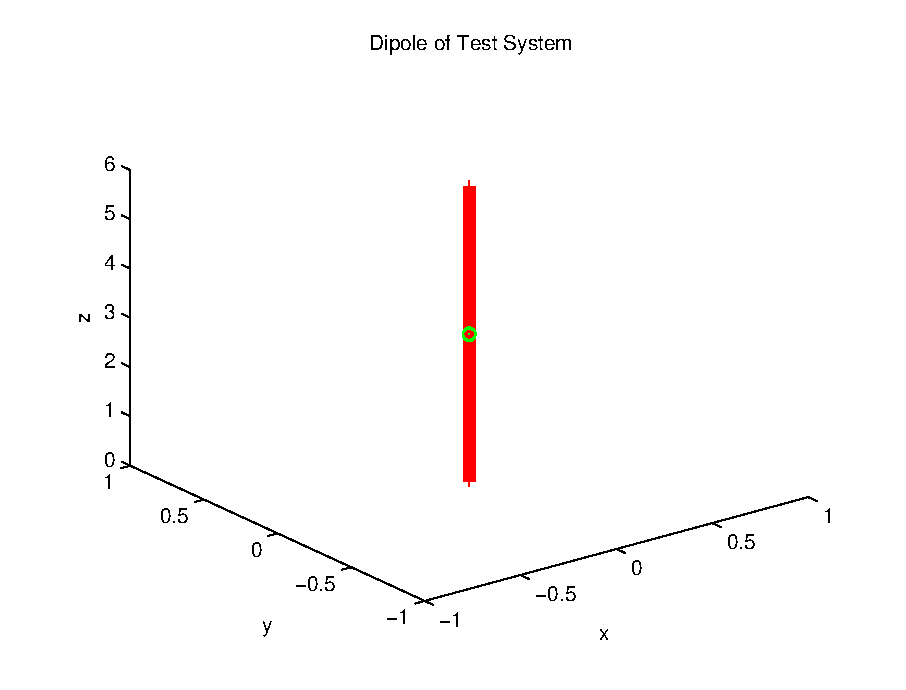
\includegraphics[width=12cm]{dipol}\\
  \caption{6 meter dipole used for calculation}\label{figDipol}
\end{figure}

\subsection{The impedances}
\begin{table}
\begin{center}
\caption{Antenna Impedances [Ohms], vacuum}
\label{tab:impedances_vacuum}
\begin{tabular}{|c|c|c|}
 \hline
 & solver 1  & solver 2  \\
\hline
$300 kHz$ & 6.3712e-03 - 3.4405e+04i &  6.4781e-03 - 3.3973e+04i \\
$1 MHz$ & 7.0845e-02 - 1.0309e+04i &  7.2034e-02 - 1.0180e+04i \\
$10 MHz$ &  7.7069e+00 - 8.8976e+02i&  7.8383e+00 - 8.7385e+02i\\
\hline
& ASAP  & Concept 2\\
\hline
$300 kHz$ &  4.3244e-01 - 3.3003e+04i &  1.4896e-02 - 3.3060e+04i\\
$1 MHz$ & 1.3959e-01 - 9.8883e+03i &  8.5201e-02 - 9.9056e+03i\\
$10 MHz$ &    7.6497e+00 - 8.5056e+02i&  7.6650e+00 - 8.5193e+02i\\
\hline
\end{tabular}
\end{center}
\end{table}




\begin{table}
\begin{center}
\caption{Antenna Impedances [Ohms], $\frac{\omega_{pe}^2}{\omega^2}=0.5$}
\label{tab:impedances_plasma}
\begin{tabular}{|c|c|c|}
 \hline
 & solver 1  & solver 2  \\
\hline
$300 kHz$ & 4.5049e-03 - 6.8814e+04i & 4.5805e-03 - 6.7950e+04i  \\
$1 MHz$ &  5.0074e-02 - 2.0632e+04i &  5.0914e-02 - 2.0372e+04i \\
$10 MHz$ & 5.2205e+00 - 1.9246e+03i &  5.3087e+00 - 1.8958e+03i \\
\hline
& ASAP  & Concept 2  \\
\hline
$300 kHz$ & 8.3245e+00 - 6.6011e+04i &  4.4189e-03 - 6.6123e+04i \\
$1 MHz$ & 5.0866e-01 - 1.9791e+04i &  4.9119e-02 - 1.9825e+04i \\
$10 MHz$ &  5.1739e+00 - 1.8435e+03i&  5.1377e+00 - 1.8466e+03i \\
\hline
\end{tabular}
\end{center}
\end{table}

Table \ref{tab:impedances_vacuum} shows the antenna impedance of the dipole at three different frequencies, computed by the two in-house-written solvers, as well as by two well proven solvers for reference. As one can see, there are some variations, especially of the resistive (real) part. The reason is that the impedance is calculated by dividing the voltage at the feed, which is 1V in this example, by the current at the feed. The current and the modeling of the excitation at the antenna feed crucially depend on the details of the implementation. For instance, the own solvers are implemented by using perfectly conducting wires, while the computations with ASAP and Concept II are performed by using a realistic conductivity. The sign of the imaginary part shows, whether the antenna behaves capacitive (-) or inductive (+).\\

Table \ref{tab:impedances_plasma} shows the impedances, calculated with the effect of the surrounding plasma included. Only the effect of the electron movement is considered and the relative permittivity has a value of $0.5$.\\

The difference between the results of different solvers is not so prominent when an integration is performed over all currents. Quantities like the effective length and the field patterns are produced by performing such an integration and usually the differences between the solvers is small in these cases.\\


\subsection{The electrical far-field-pattern}
Field patterns are a very good way to visualize direction dependent properties of a receiving or transmitting antenna. There are many different types of patterns, all serving the purpose of this paper. Here the electric far field patterns are presented, normalized to a factor of $\frac{e^{\imath \mathbf{k}\cdot \mathbf{r}}}{r}$, where $\mathbf{r}$ is the vector from the phase center of the antenna to the observing point, and $\mathbf{k}$ the wave vector. Hence, to get the magnitude of the physical field, the presented value has to be multiplied by this factor.\\

\begin{figure}
  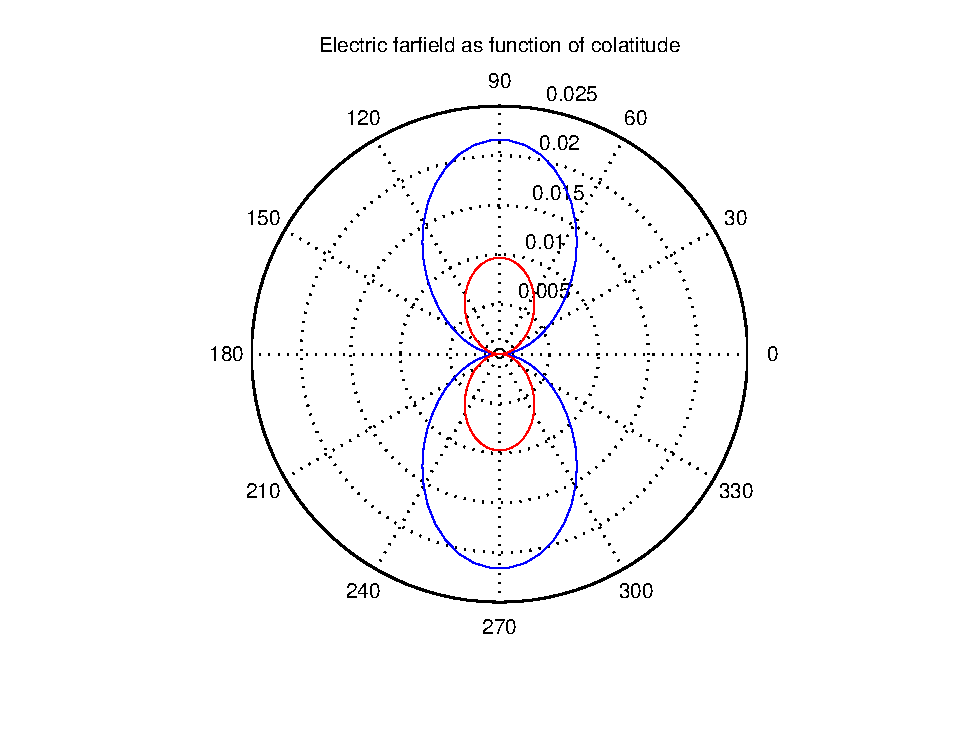
\includegraphics[width=12cm]{ff_10mhz.eps}
\caption{Electric far-field-patterns for the 6m dipole in vacuum (blue) and in plasma (red), computed with solver 2.}
\label{fig:patterns_vacuum}
\end{figure}

Figures \ref{fig:patterns_vacuum} show 2-dimensional plots of the electric far-field pattern of the 6m dipole at $10 MHz$ in vacuum (upper figure) and in isotropic cold plasma, using a relative permittivity of 0.5. The result is in perfect agreement with the results when computed with Concept II and with theory. The radiated field in plasma is lower than in vacuum. in this configuration the difference is approximately 1 order of magnitude. The physical reason is that part of the transmitted energy is stored in the oscillating motion of the plasma particles. This energy is often called ordered kinetic energy. In this case only electrons are considered, when considering also ions, the magnitude of the respective values of the pattern is even lower by a small amount. The difference is so small that the effect of the ions can be neglected in this case.

\subsection{The effective length vectors}
A very useful antenna property which describes the behavior of a transmitting antenna is the effective length vector. It can be computed as

\begin{equation}
\textbf{h}_{eff}=\frac{1}{I}\int \mathbf{J}(\mathbf{r}')e^{\imath \mathbf{k} \cdot \mathbf{r}'} dV'
 \end{equation}

$I$ is the feed current. In general it is complex and depends upon direction of the incident wave. These dependencies can safely be neglected at low frequencies, i.e. the quasistatic range, where the effective length vector can be regarded as real and constant. This range can be estimated for spacecraft to exist up to frequencies where the wavelength can still be regarded as large in relation to the spacecraft and antenna dimensions. It is a well-known result of antenna theory, that the effective lengths of an ideal dipole is half its physical length. Real antennas, especially spacecraft antennas behave slightly different. The reasons for this deviation from ideal conditions can be found in the shape of the spacecraft body, the base capacitances, the finite diameter of a real antenna, and, as will be shown below, the surrounding space plasma.\\

When using computed effective length vectors for analyzing data, one should keep in mind that they are results of calculating transmitting antennas. In vacuum they can be used to describe receiption properties of antennas due to the principle of reciprocity. This principle is not directly valid in a plasma environment, so the meaning of the effective length vector in plasma has to be investigated.\\


\begin{table}
\begin{center}
\caption{Effective length vectors in vacuum [m]}
\label{tab:heff_vacuum}
\begin{tabular}{|c|c|c|c|}
 \hline
 & solver 1  & solver 2  & Concept 2 \\
\hline
$300 kHz$ & 2.842 & 2.864 & 2.812 \\
$1 MHz$ & 2.843 & 2.866 &  2.813 \\
$10 MHz$ & 2.985 & 3.010 &  2.863  \\

\hline
\end{tabular}
\end{center}
\end{table}

\begin{table}
\begin{center}
\caption{Effective length vectors in plasma [m]}
\label{tab:heff_plasma}
\begin{tabular}{|c|c|c|c|}
 \hline
 & solver 1  & solver 2  & Concept 2 \\
\hline
$300 kHz$ & 2.842 & 2.864 & 2.812  \\
$1 MHz$ & 2.842 & 2.865 & 2.812  \\
$10 MHz$ & 2.912 & 2.935 & 2.813 \\

\hline
\end{tabular}
\end{center}
\end{table}

Tables \ref{tab:heff_vacuum} and \ref{tab:heff_plasma} show the lengths of the effective length vectors of the dipole under the specified conditions. The direction of the wave was always taken to be the positive x-axis, i.e. perpendicular to the dipole. Investigations have shown that the dependence of the effective length vector is only very small at the frequencies where calculations were performed.\\

Only the real part is presented here. Since the direction of the effective length vector of a straight dipole is always in the direction of the dipole, there is no need to present the vectors in vector form.\\

As it can be seen, the effect of the plasma is a shortening of the effective length vectors. Although the effect is quite small in the presented data, as well as under most realistic conditions, it is generally true.\\

In the stable frequency range, the relation between the equivalent permittivity and the length of the effective length vector is nearly linear for a dipole. For more complex structures, like real spacecraft, this is not generally true. The proportionality factor for the near-linear behavior depends on the frequency. Figure \ref{fig:relative_heff_shortening} shows the equivalent length of the effective length vector as a function of equivalent permittivity for 3 frequencies. The calculation was performed with solver 2 and Concept II. It can clearly be seen that the most prominent effect of the isotropic plasma on the effective length vector is at the highest frequency.\\

\begin{figure}
  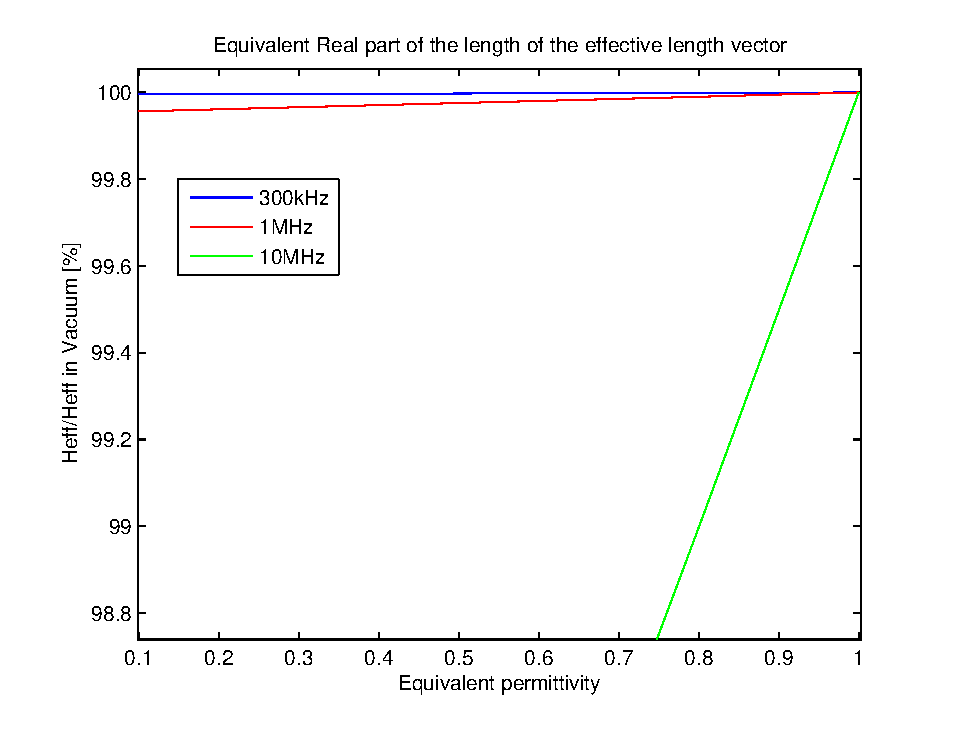
\includegraphics[width=12cm]{heff_shortening_dipole.eps}
\caption{Equivalent length of the effective length vector in relation of vacuum case, as a function of equivalent permittivity.}
\label{fig:relative_heff_shortening}
\end{figure}

\subsection{Impedance patterns}
Figures \ref{fig:impedances_dipole_solver2_real} and \ref{fig:impedances_dipole_solver2_imag} show the real and the imaginary parts of the antenna impedances as a function of frequency. The frequency range is from $100kHz$ to $100MHz$. The results of the calculation for vacuum are plotted in blue, while the plasma case is plotted in red. For these two Figures a constant equivalent permittivity of 0.5 was used. This situation is unrealistic, but we only want to demonstrate the effect of the plasma in the numerical simulation.\\

As it can be seen, the antenna resonances, the frequencies where the imaginary part of the impedance vanishes, are shifted to a higher frequency This corresponds to the effect to be expected for a shorter effective length vector. The plasma effect increases with increasing frequency.\\

Knowledge of the antenna resonances is of vital importance for the correct interpretation of measured data of radio experiments on spacecraft. Especially the even numbered resonances where the imaginary part of the impedance crosses the zero line from the positive to the negative area corresponds to a peak of the curve of the real part and in vicinity of this peak the effective length vectors computed by numerical means can not be considered as reliable. Therefore the inclusion of the plasma effect in numerical calibration can be considered as important, also at radio frequencies.\\


\begin{figure}
  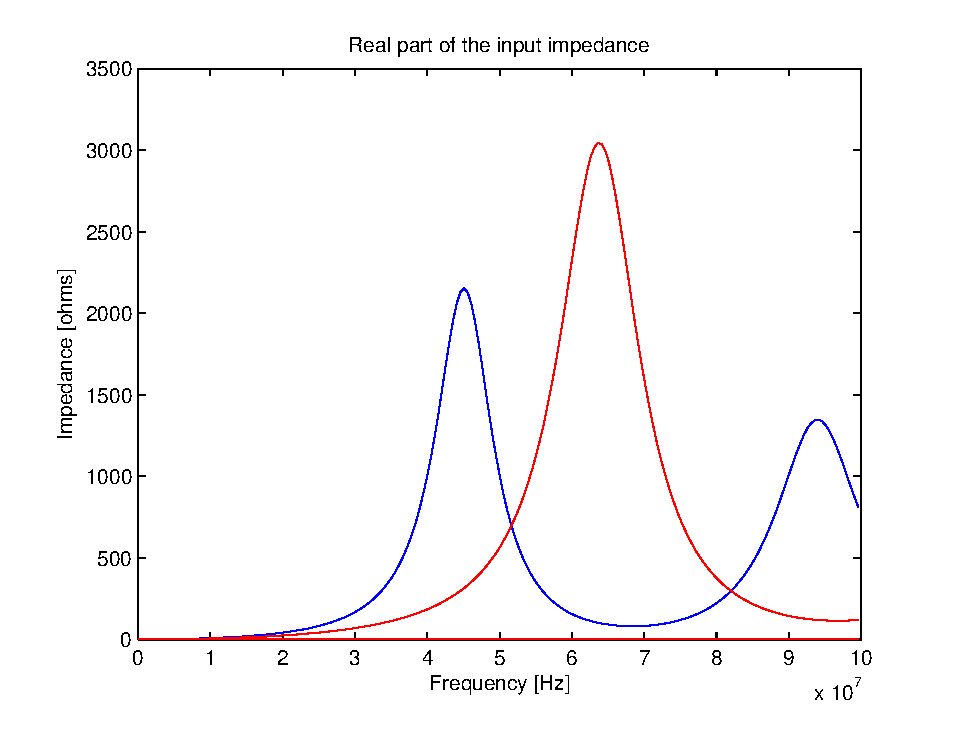
\includegraphics[width=12cm]{imps_dipole_solver2_real.eps}
\caption{Real part of 6m dipole impedance, from $0.1 - 100 MHz$, computed with solver 2. The blue line shows the impedance in vacuum, whereas for the red line $\epsilon_r$ was held constant at $0.5$.}
\label{fig:impedances_dipole_solver2_real}
\end{figure}

\begin{figure}
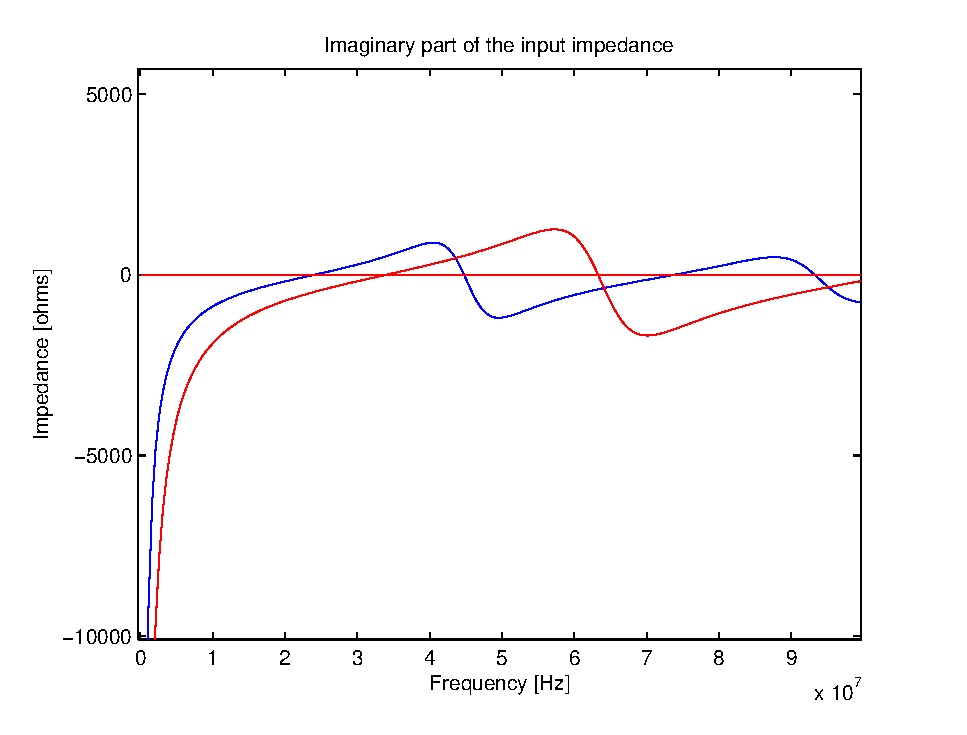
\includegraphics[width=12cm]{imps_dipole_solver2_imag.eps}
\caption{Imaginary part of 6m dipole impedance, from $0.1 - 100 MHz$, computed with solver 2. The blue line shows the impedance in vacuum, whereas for the red line $\epsilon_r$ was held constant at $0.5$.}
\label{fig:impedances_dipole_solver2_imag}
\end{figure}

The realistic case is more subtile. Figures \ref{fig:impedances_dipole_solver2_real2} and \ref{fig:impedances_dipole_solver2_imag2} show a similar calculation, but this time the plasma electron frequency was set to $10MHz$, a situation which could be realistic in some dense plasma environments in space, as in the ionosphere. The frequency range in these figures is from $10.1$ to $100MHz$. The differences between vacuum and plasma are smaller and decrease with higher frequency. The electron plasma frequency is a cutoff, where the imaginary part of the antenna impedance tends to minus infinity and no electromagnetic radio waves can propagate.

\begin{figure}
  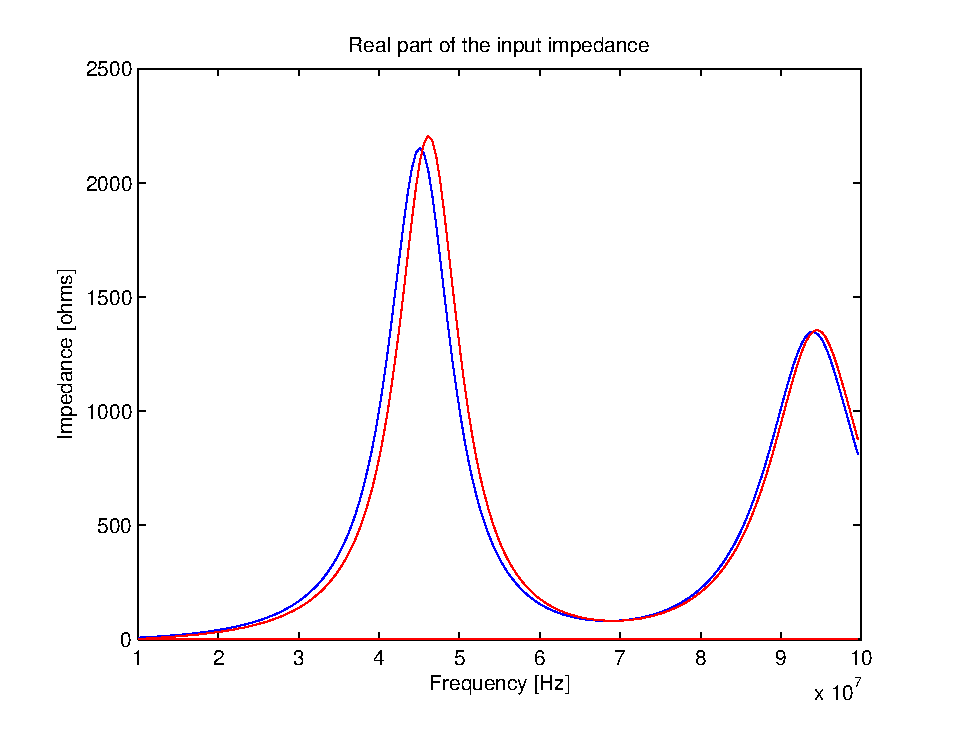
\includegraphics[width=12cm]{imps_dipole_solver2_real2.eps}
\caption{Real part of antenna impedance, $10.1 - 100 MHz$, computed with solver 2. $f_p=10MHz$.}
\label{fig:impedances_dipole_solver2_real2}
\end{figure}

\begin{figure}
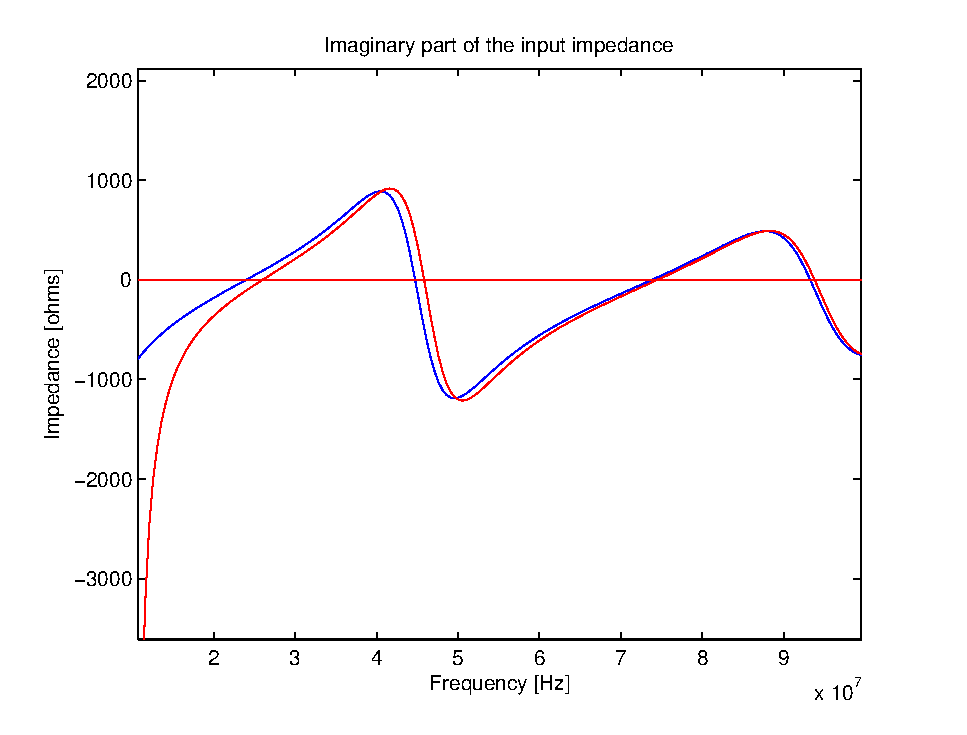
\includegraphics[width=12cm]{imps_dipole_solver2_imag2.eps}
\caption{Imaginary part of antenna impedance, $10.1 - 100 MHz$, computed with solver 2. $f_p=10MHz$ was held constant at $0.5$.}
\label{fig:impedances_dipole_solver2_imag2}
\end{figure}

\section{Application to a real spacecraft (STEREO)}
In this section the effect of space plasma will be included in the calculation of antenna properties of actual spacecraft antennas. This is only performed for cold isotropic plasma, by using the Concept II solver and the method of encapsulating the plasma effects in the equivalent dielectric function as presented before. General purpose solvers being capable of handling magnetized plasma and complicated 3D spacecraft structures, are not available to the knowledge of the authors. A respective solver will be implemented by the authors in the near future and be presented in a subsequent publication. \\

The spacecraft upon which the calculations are applied is the STEREO A spacecraft. The reason for this is that there exists a good wire and patch model as well as experimental results and actual measured data. Additionally the authors of this paper have some experience with regard to antenna calibration with this spacecraft \cite{ossi09} and \cite{panchenko10}. The respective wire/patch grid model is shown in Figure \ref{fig:stereo}.\\

\subsection{The STEREO mission and the WAVES experiment}
On October $25^{th}$, 2006, NASA launched the two STEREO spacecraft with a radio experiment on board, called STEREO-WAVES (S/WAVES), which is designed to observe solar radio emissions by using direction finding capabilities. The S/WAVES experiment is designed to track solar and interplanetary radio bursts and trace the generation and evolution of radio disturbances from the Sun to Earth orbit and beyond. Each spacecraft has three nearly orthogonal antennas, capable of receiving electromagnetic waves in several frequency ranges. The main operational range of the receivers is between 10kHz and 16MHz. With this configuration, it is possible to perform goniopolarimetry at the lower end of the frequency range to determine the direction of incidence and the polarization of the received radiation. When both spacecraft receive radiation from the same source, the actual location of the source can be pinpointed by the method of triangulation.\\

For the correct interpretation of the data it is of vital importance to know the antenna properties with great accuracy. Numerical and experimental antenna calibration was performed by the Radio Group of the Space Research Institute of the Austrian Academy of Sciences, based in Graz. During these calibrations, which are published in \cite{ossi09} and \cite{macher07} a vacuum environment was postulated. In this section the effect of an isotropic plasma on the results of the numerical calibration will be discussed.\\

\begin{figure}
\begin{center}
\includegraphics[width=14cm]{stereo.eps}
  \caption{The STEREO spacecraft wiregrid}\label{fig:stereo}
\end{center}
\end{figure}

The STEREO/WAVES experiment works with three mutually orthogonal stacer
monopole antennas. This paper applies to the HFR and band B and C of the LFR. The HFR operates in a range from 125 kHz to 16.025 MHz. The HFR provides all auto- and cross-correlation parameters. Two direction finding (DF) modes are implemented, one of which uses the antennas as dipoles. The other DF mode uses
the antennas as monopoles. The HFR is a sweeping frequency receiver and each sweep takes approximately 15 seconds. Only the monopoles are treated in this article.\\

Bands B and C provide auto- and cross-correlation parameters and can be used
for DF.\\



\subsection{The effect on the antenna impedances}

\begin{figure}
\begin{center}
  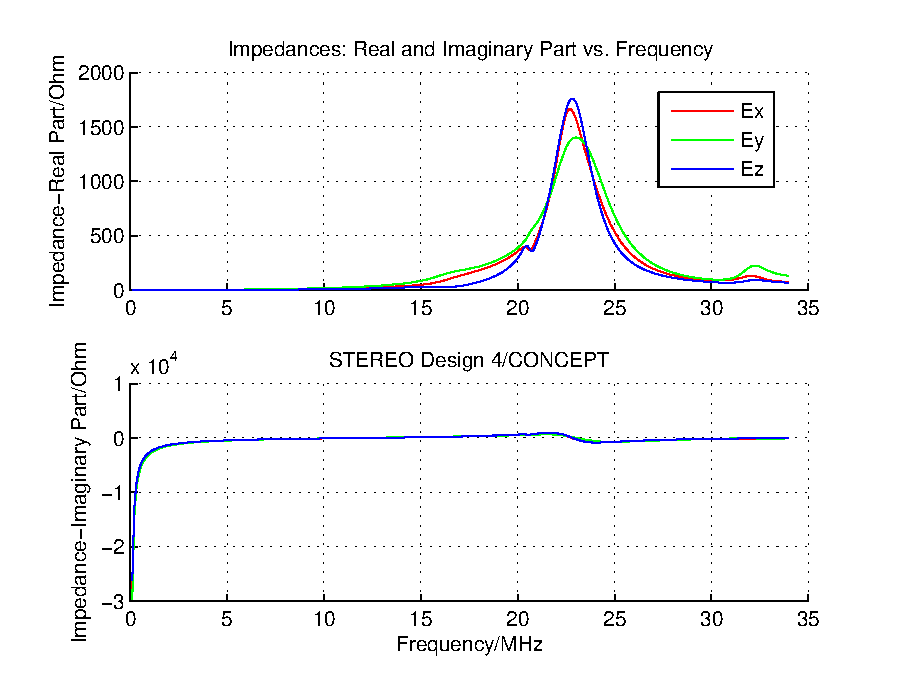
\includegraphics[width=11.5cm]{impedance_stereo_vac.eps}
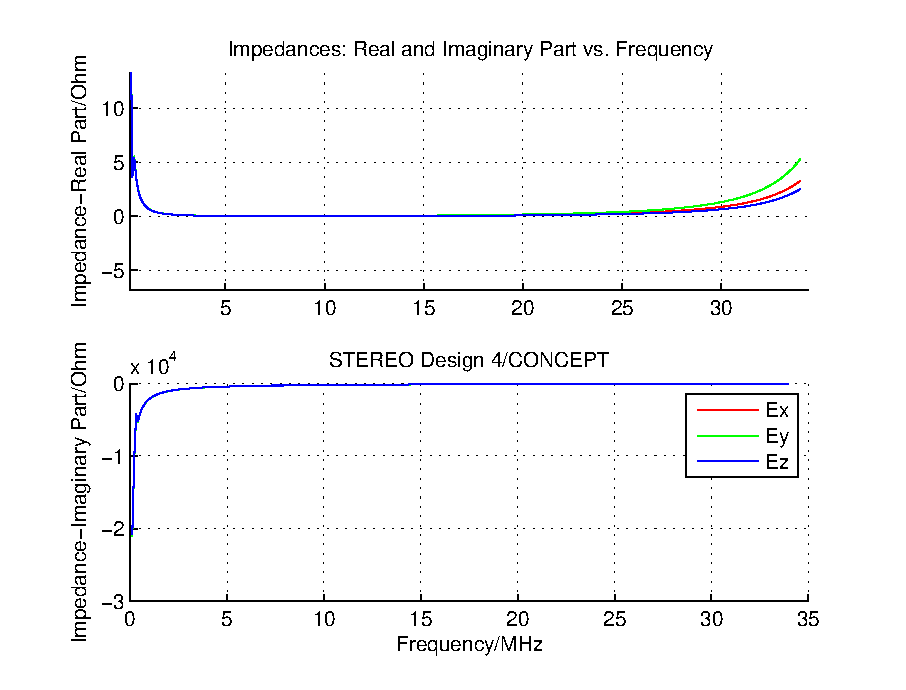
\includegraphics[width=11.5cm]{impedance_stereo_pl.eps}
  \caption{The impedance of the S/WAVES antennas in vacuum (top) in relation to cold plasma with $\epsilon_r=0.1$ (bottom)}\label{fig:imp_stereo}
  \end{center}
\end{figure}

Figure \ref{fig:imp_stereo} shows the results of these calculations, performed with a constant equivalent permittivity of $0.1$, again for demonstration purposes. The effect on the impedance curve shows the same behavior as for the dipole. The resonance is shifted to a higher frequency. The curves for the three antennas are so close together at some parts, that they appear as single line. Since Matlab draws one line after another, the final color of the line is blue, the color of the last curve to be drawn on top of the others. The same is true for the following figures.\\

\begin{figure}
\begin{center}
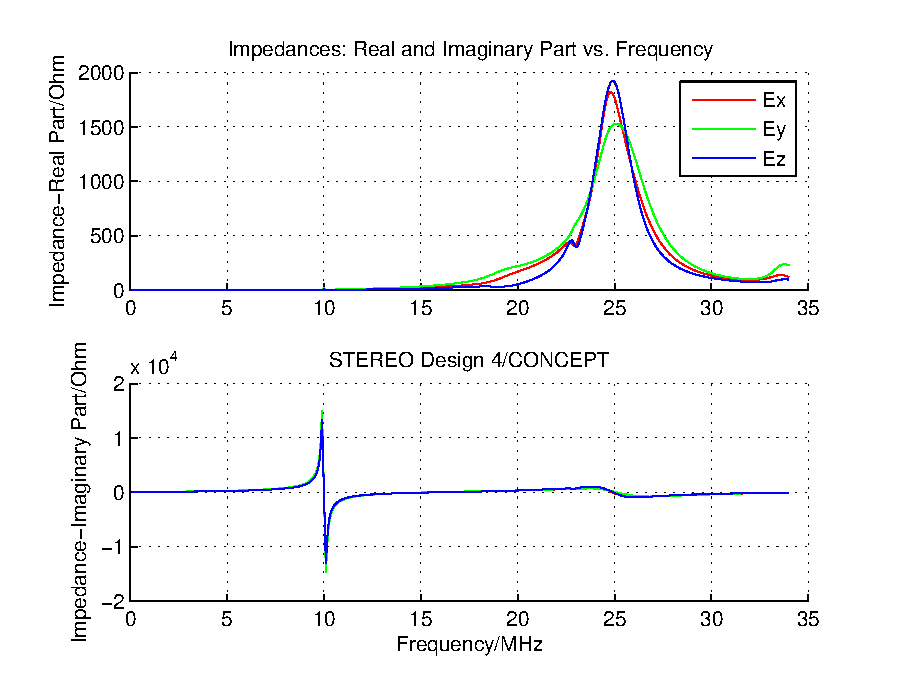
\includegraphics[width=11.5cm]{impedance_stereo_pl_fix.eps}
  \caption{The impedance of the S/WAVES antennas in cold plasma with $f_{pe}=10MHz$ (bottom)}\label{fig:imp_stereo_fix}
  \end{center}
\end{figure}

Figures \ref{fig:imp_stereo_fix} show the same calculation with a fixed electron plasma frequency of 10MHz. Only the part of the graph above 10MHz is relevant. The calculation is not valid at the lower frequency range.\\

One can see the shift of the second antenna resonance due to the influence of the plasma. Even on the realistic plot with the fixed plasma frequency, the peak of the real part of the impedance curve is shifted by more than 2 MHz. STEREO will not have to deal with conditions where such high plasma frequencies exist, but for other space missions taking measurements inside the ionosphere, or, although with lower resonance frequencies, in planetary Magnetospheres, such shifts should be take into account.\\

The plasma frequency is

\begin{equation}\label{Plasma frequency}
    f_p=\sqrt{\frac{1}{2\pi}{\frac{n_e e^2}{ m \epsilon_0}}}
\end{equation}

At conditions where STEREO operates, i.e. at 1AU in interplanetary space, which corresponds roughly to an electron plasma frequency between 20kHz and 60kHz, we will set the electron plasma frequency to a rounded value of 100kHz. Figure \ref{fig:imp_stereo_fix_100kHz} shows the result. To the resolution of this figure, there is no visible difference to the vacuum computation. Hence, it seems that the plasma effect can be neglected for the calculation of the impedance curves and the estimation of the antenna resonances of the radio experiment of the STEREO spacecraft.


\begin{figure}
\begin{center}
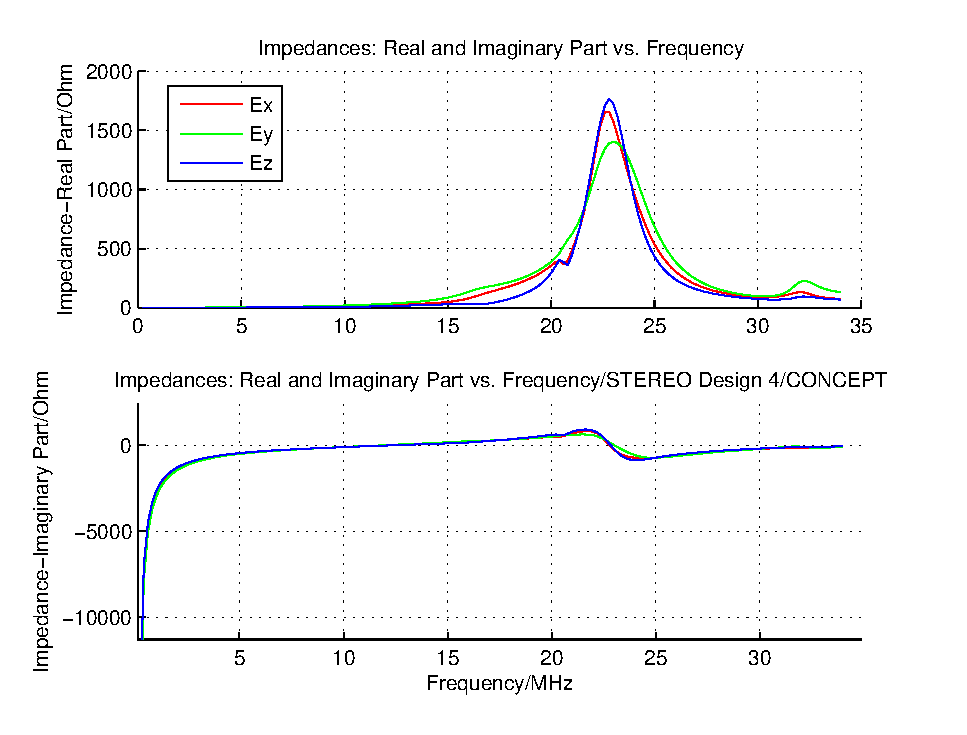
\includegraphics[width=11.5cm]{impedance_stereo_pl_100khz.eps}
  \caption{The impedance of the S/WAVES antennas in cold plasma with $f_{pe}=100kHz$ (bottom)}\label{fig:imp_stereo_fix_100kHz}
  \end{center}
\end{figure}

\subsection{The effect on the effective length vectors}
Computing the effective length vectors using the cold plasma permittivity results in a slightly shorter effective length vector. The directions are not altered very much. As an example the quasistatic effective length vectors of the STEREO antennas are given in Tables \ref{tab:heff_vacuum_stereo} and \ref{tab:heff_cold_plasma_stereo}. In both cases a frequency of $300kHz$ is used, which is a typical value when investigating the behavior of an antenna in the quasistatic limit. At the first table, vacuum is used as the surrounding medium, while a cold isotropic plasma model is used for comparison (Table \ref{tab:heff_cold_plasma_stereo}), using again the realistic value of 100kHz as electron plasma frequency.\\

Plasma frequency and wave frequency are close togeather in this example, so the difference in length of the effective length vectors is clearly visible (about 10cm) and should be considered for data processing of the measured S/WAVES data.

The coordinate frame used for presenting the effective lengths vectors is a spherical polar coordinate frame with the principal axes point towards the x-axis, i.e. the direction of the sun. The coordinates of the physical antennas are shown in Table \ref{tab:phys_ant}. Details can be found in \cite{ossi09} \\

For the calculations, base capacitances of $70pF$ where used. The inclusion of base capacitances has also the effect of decreasing the lengths of the effective length vectors.\\


\begin{table}
\begin{center}
\caption{Effective length vectors in vacuum: $f=300kHz$}
\label{tab:heff_vacuum_stereo}
\begin{tabular}{|c|c|c|c|}
 \hline
 & $length/m$ & $\zeta/^\circ$ & $\xi/^\circ$ \\
\hline
$E_x$ & $1.35$ & $119.9$ & $-135.3$ \\
$E_y$ & $1.64$ & $114.4$ & $127.3$ \\
$E_z$ & $1.09$ & $124.7$ & $15.5$ \\
\hline\end{tabular}
\end{center}
\end{table}



\begin{table}
\begin{center}
\caption{Effective length vectors in cold plasma: f=300kHz, $f_{pe}=100kHz$}
\label{tab:heff_cold_plasma_stereo}
\begin{tabular}{|c|c|c|c|}
 \hline
 & $length/m$ & $\zeta/^\circ$ & $\xi/^\circ$ \\
\hline
$E_x$ & $1.26$ & $119.6$ & $-135.0$ \\
$E_y$ & $1.53$ & $114.1$ & $127.2$ \\
$E_z$ & $1.02$ & $124.3$ & $15.2$ \\
\hline\end{tabular}
\end{center}
\end{table}

\begin{table}
\begin{center}
\caption{Physical antennas}
\label{tab:phys_ant}
\begin{tabular}{|c|c|c|c|}
 \hline
 & $length/m$ & $\zeta/^\circ$ & $\xi/^\circ$ \\
\hline
$E_x$ & $6.00$ & $125.3$ & $-120.0$ \\
$E_y$ & $6.00$ & $125.3$ & $120.0$ \\
$E_z$ & $6.00$ & $125.3$ & $0.00$ \\
\hline\end{tabular}
\end{center}
\end{table}

Figure \ref{fig:relative_heff_shortening_stereo} shows the equivalent reduction of the length of the effective length vector in relation to the vacuum case as a function of the equivalent permittivity for all three STEREO/WAVES antennas at a frequency of 300kHz. It can be seen that the relative shortening is far more pronounced than for the dipole. This graph can be used to estimate the plasma effect on the effective length vectors for calibration purposes. Similar figures can easily be produced for a selection of frequencies.\\

\begin{figure}
  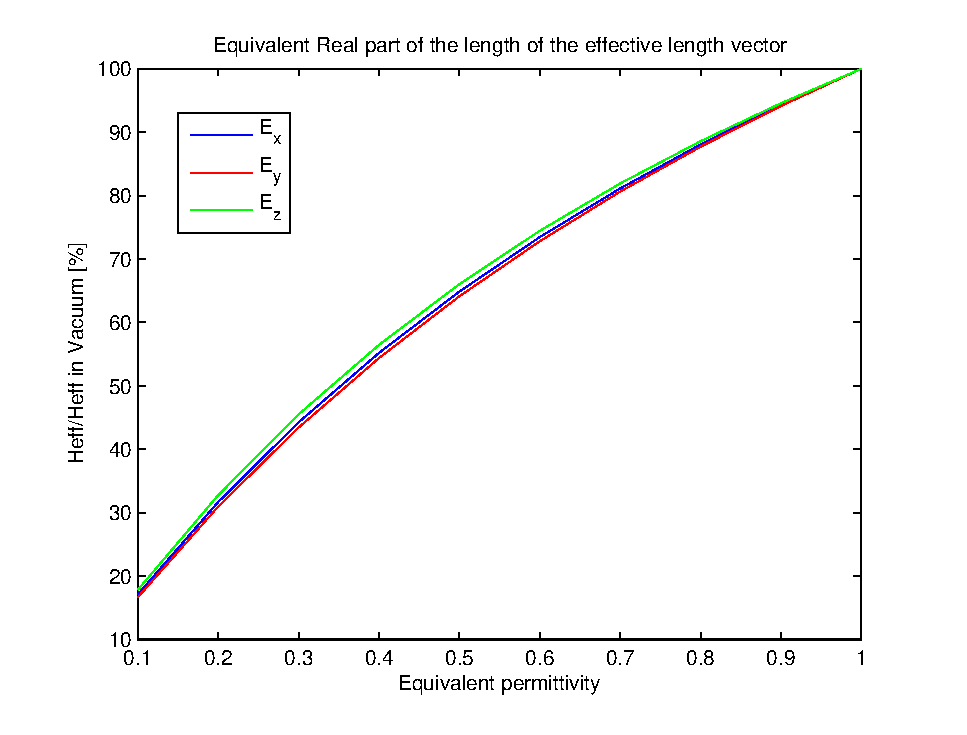
\includegraphics[width=12cm]{heff_shortening_stereo.eps}
\caption{Equivalent length of the effective length vector in relation of vacuum case, as a function of equivalent permittivity.}
\label{fig:relative_heff_shortening_stereo}
\end{figure}


\section{Conclusion}
In this article, the effect of plasma on spacecraft antenna properties was investigated. On a theoretical basis a method was shown, how the plasma effect can be incorporated into numerical antenna calibration. It was also shown that a simple model of cold plasma is valid for this task. Kinetic, relativistic or quantum mechanical treatment is not necessary.\\

Two simple solvers were implemented, using a boundary element method known as Method of Moments, to solve the electric field integral equation for computing the current distribution along a dipole. For validation, the results where compared to the results of 2 well proven solvers, one open source software called ASAP, and one proprietary program, called Concept II.\\

Using these solvers, simple calculations of antennas in isotropic plasma where performed and studied. Then calculations where performed for antennas of a real space radio experiment, S/WAVES mounted on the STEREO spacecraft. It was shown that the effects of the plasma in interplanetary space at approximately 1AU, i.e. the regime where STEREO operates, are so small they can be neglected for certain applications. The effect of the the plasma on the effective length vectors in the quasistatic range is present, however (approximately 10cm) and should be considered for data interpretation. For space missions operating in different regimes, especially in the ionosphere, the effect of plasma on the antenna properties in the radio frequency range could be more dramatic, which make a careful analysis mandatory.\\



\bibliography{../../Bibliography/MyBib2}
\bibliographystyle{agu04}

\end{document}
